\section{Introduction}
The Minimum Vertex Cover (MVC) problem seeks to find a subset of vertices for a given graph G such that all the said vertices touch all edges of the graph. This is a well known NP Complete problem that has many real world applications including finding phylogenetic trees based on protein domain information \cite{abu2004kernelization} or finding where to place bunkers to cover all cities. For this project, our group was tasked with solving the MVC problem using three different approaches: branch-and-bound, local search, and approximation. 

\subsection{Approximation Algorithm}
The approximation approach is one that sacrifices accuracy of the result in favor of speed. Generally, approximation algorithms have a provable guarantee that they will be no worse than $p\left( n \right)\times OPT$, where $p\left( n \right)$ is some value greater than or equal to 1 that may depend on the size of the problem and OPT is the optimal solution. For the MVC problem, the approximation approach involves arbitrarily picking an edge in the given graph, then removing is and all neighboring edges from the graph. Then a new edge is arbitrarily picked from the remaining ones and the process is repeated until all the edges have been removed. The vertex cover will then be the nodes corresponding to all the arbitrarily picked edges.

\subsection{Local Search}
In addition to the traditional hill climbing approach, the local search I algorithm has options such as forward stopping when the optimal vertex count is reached, remembering the best solution obtaining so far, growing and shrinking (either direction traversal). The local search approach begins with an initial solution and then tries to obtain the global minima by choosing neighbours and moving to the neighbour with the best eval function. The eval function for the local search approach is the number of edges incident on the vertex that is to be added to the current set of vertices in our current search iteration.

\subsection{Branch and Bound}
Branch and bound algorithm derives from backtracking strategy for decision problems, which iterates through all the possible solutions in the search space and eliminates some unpromising alternatives from consideration. Branch and bound further refines this idea for optimization problems. It keeps the best solution found so far and computes a lower bound based on this solution. When a solution node for a sub-problem is worse than the lower bound, we consider it as an unpromising solution node and prune it and all its child nodes. Although branch and bound algorithm is a general idea for NP-complete problems, how to compute the lower bound has to be customized for each individual application. This strategy reduces the time consumption on searching for solutions and a global optimal solution is guaranteed, but the worst case is still exponential. Therefore, this algorithm can be useful only when the instances are small.

\section{Problem}
Consider a graph $G=\left( V,E \right)$.  Formally, a vertex cover ${V}'$ is a subset of $V$ such that for each $\left( u,v \right)\in E$ it follows that either $u\in{V}'$or $v\in{V}'$. This set ${V}’$ is said to cover the edges of $G$. For the project at hand, this problem is further complicated by searching for the smallest possible ${V}’$ that satisfies the above definition. The MVC problem is known to be NP Complete, and as such it requires specialized algorithms such as local search and approximation in order to be solved. 

\section{Algorithms}
\subsection{Approximation Algorithm}
As mentioned above, the approximation algorithm works by arbitrarily picking an edge in the graph, adding its nodes to the solution, then removing the edge and all of its neighboring edges from the graph, and repeating this process until all edges have been removed. In pseudocode, this looks like the following:

\begin{algorithm}[ht]
\SetAlgoNoLine
$C = \{ \}$\;
$E^{\prime}= E$\;
\While{$E^{\prime}$ is not empty}{remove $e$ in $E^{\prime}$ and add its nodes to $C$\;
		remove all edges neighboring $e$ from $E^{\prime}$\;
}
return $C$\;
\caption{MVC Approx($G$)}
\label{alg:one}
\end{algorithm}

This algorithm is inspired by that found in CLRS Chapter 35. The algorithm works by choosing an edge arbitrarily, then adding its nodes to the solution and removing all edges neighboring said nodes. This is done because the nodes added to the solution now cover all the edges, so they do not need to be considered. By repeating this process until every edge has been removed from the graph, this guarantees that the solution will cover all edges in the graph by design. This algorithm is provably a 2-approximation algorithm, which means that any solution found will be no worse than twice the size of the optimal solution. 

Because of its structuring, it is not particularly complex and thus fast compared to the other algorithm options. But it also does not give exact solutions except for particular cases, which can be disadvantageous depending on the application of it. As seen in the table below, the approximation algorithm runs extremely quickly, but has high relative error. 

\subsection{Local Search Algorithm I: Initial Solution and approach}
The local search is capable of traversing two ways:

\begin{enumerate}
\item When the vertices in the current search iteration form a vertex cover, we try to remove a vertex so as to see if a lesser size vertex cover is possible

\item When the vertices in current search iteration do not form a vertex cover, we try to add a maximum impact vertex from a random uncovered edge and perform the check for vertex cover once again.
\end{enumerate}
\begin{algorithm}[ht]
\SetAlgoNoLine
\KwIn{graph $G = (V, E)$, no\_of\_iterations}
\KwOut{vertex cover of $G$ \textbf{if} k = no of vertices \textbf{else} optimal vertex coverage obtained so far}
{gain(v) := no of edges for each vertex $v \in G$\;
Circ\_deque\_len = circular deque of length 100\;
C := ConstructVC(k) // constructs list of size k with vertices sorted according to no of edges incident on them\;
\While{time > cutoff}{
\If{Edge\_set == total\_no\_of\_edges}{
Circ\_deque\_len.append(C.length)\;
\If{length of C is the minimum length in Circ\_deque\_len}{
Optimal\_soln = C\;}
remove a random Vertex from C and update Edge Set\;
Continue\;}
U,V = vertices of a random uncovered edge \;
Append either U/V to C depending on the number of edges incident on U,V and update Edge Set\;
Return Optimal\_soln or C if Optimal soln is empty\;
}
}
\caption{LocalSearch(G , cut\_off, seed)}
\end{algorithm}

Here the maximum impact vertex is the vertex with most edges incident on it. Random uncovered edge is chosen from the set of edges in the graph that do not have any of its vertices on the current iteration of VC. In order to get a guaranteed VC, we can start with initial solution equal to the total number of vertices and the minimum impact vertices are removed. However, for large graphs this can be quite time consuming - for each VC of specific length almost all other possible permutations are tried. Thus the rate at which the VC size decreases is very low. The optimal strategy is to begin with $\frac{\left| V \right|}{2}$ vertices which have the maximum impact which is done in the method ConstructVC. The current iteration vertices list will grow to add more vertices if a VC is not currently found.
\subsection{Local Search Algorithm II: Simulated Annealing with random restart}
Neighbourhood choice: Choosing a vertex with more number of edges incident to them does not necessarily ensure edge coverage. The second approach allows us to add the vertex with lesser number of edges incident on them with a specific probability. With Simulated Annealing, we can allow exploration at lower temperatures(more chances of adding vertices with lesser vertices incident on them) and at higher temperature, there is more exploitation of the gradient. Thus the probability of choosing a vertex with lesser number of edges incident on them is:
\begin{equation}
P\left( C,n \right)=\frac{1}{1+{{e}^{\frac{\Delta E}{T}}}}
\end{equation}

Where $n$ is the next vertex to be added to current VC vertices. $\Delta E$ is the number of edges additionally covered by adding $n$. $T$ is temperature.

This algorithm is different from the previous algorithm because of the neighbourhood choice. The algorithm makes note of edges $(u,v)$ that have both $u$ and $v$ in VC and attempts to remove one of the vertices from the vertex cover.

\begin{algorithm}[ht]
\SetAlgoNoLine
Construct\_VC\_2(K): // function called\;
Return top K vertices with most edges adjacent on them\;
//main body\;
T <- very - high\;
K = 0.65 * $|V|$ // Choose about 65\% of all the vertices\;
C <- Construct\_VC\_2(K)\;
\While{T}{Monotonically decrease T\;
\If{VC is not obtained}{
n <- random\_neigh(C)\;
Evaluate $\Delta E$\;
Evaluate $P(C,n)$\;
Add n to C with probability $P(C,n)$\;}
\If{VC is obtained}{
Maintain a list of edges (u,v) such that it has both u and v in the current VC\;
Randomly remove one of the vertices\;
}}
\caption{Local Search(G, cut\_off, seed)}
\end{algorithm}
\subsection{Branch and Bound}
Branch and bound algorithm keeps the best solution found so far and computes a lower bound based on this solution. When a solution node for a sub-problem is worse than the lower bound, we consider it as an unpromising solution node and prune it and all its child nodes. The solution tree represents all the possible solutions. A sample solution tree for a graph with 4 vertices is given below. When we scan through all the nodes, a lower bound is calculated to determine whether a node and its branch is promising or not. If it is not a potential solution, we will skip this branch and continue our scan.

\begin{figure}[ht]
  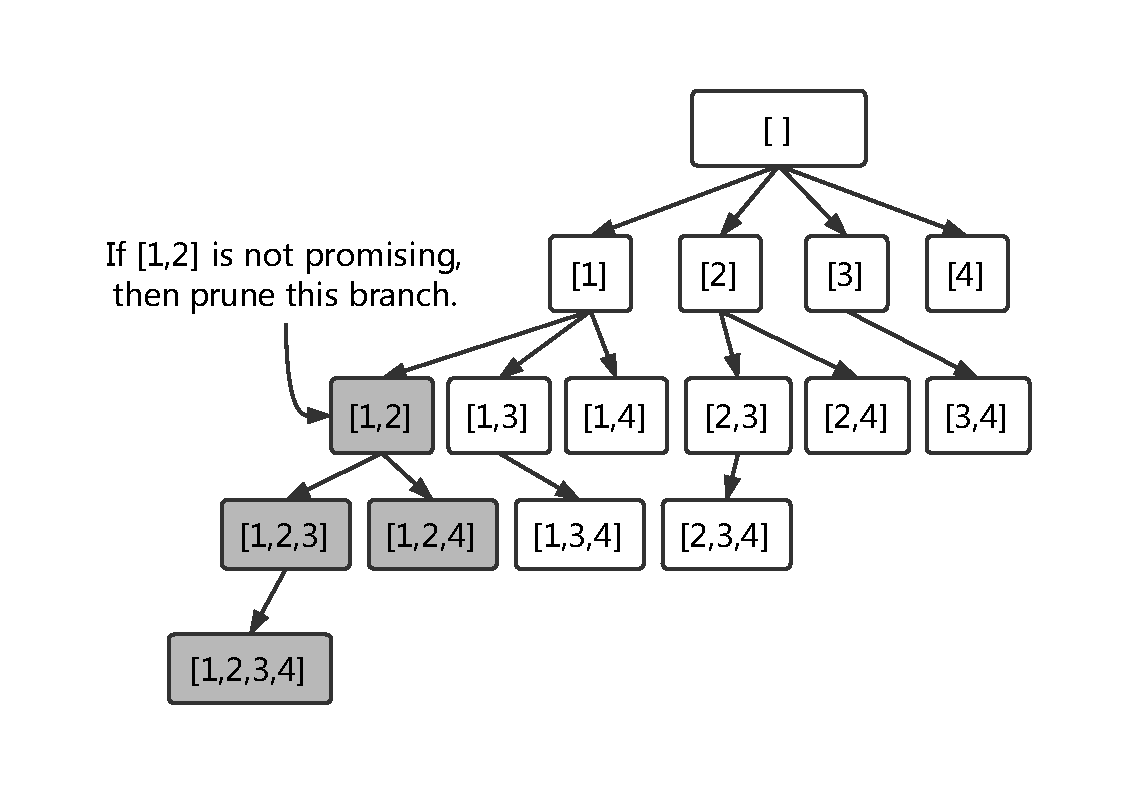
\includegraphics[scale=0.5]{tree}
  \caption{Sample solution tree for a graph with four vertices}
  \label{fig:one}
\end{figure}

\begin{algorithm}[ht]
\SetAlgoNoLine
Bnb(): //main body\;
\If{len of result + lowerbound() >= len of min so far}{return\;}
\eIf{it is a better global solution}{Record it as min so far\;Return\;}
{\For{all the left items}{Add it in the solution\;Call Bnb()\;Remove it in the solution\;}
}
Lower bound(): //function to compute the lower bound\;
LB = 0\;
\While{True}{Randomly remove two nodes in the same edge\;LB ++\;
\If{G has no edge left}{return LB\;}
}
\caption{Branch and bound}
\end{algorithm}
\section{Empirical Evaluation}

For the approximation algorithm as well as the local search 1, all computations were run on a late 2013 15 inch MacBook Pro with 2.3 GHz Intel Core i7 and 16 GB of 1600 MHz DDR3 RAM. 

\subsection{Approximation Algorithm}
See Table \ref{tab1} for comprehensive evaluation for approximation algorithm.
\begin{table}[htb]
\caption{Comprehensive evaluation table for approximation algorithm}
\label{tab1}
\begin{minipage}{\columnwidth}
\begin{center}
\begin{tabular}{@{}lllll@{}}
\toprule
Graph        & OPT  & Approx. & Time (s) & Error \\ \midrule
Jazz         & 158  & 186     & 0.094    & 0.18  \\
Karate       & 14   & 22      & 0.00069  & 0.57  \\
Football     & 94   & 110     & 0.017    & 0.17  \\
as-22july06 & 3303 & 6026    & 163.91    & 0.82  \\
hep-th       & 3926 & 5784    & 51.85    & 0.47  \\
Star         & 6909 & 10536   & 268.38    & 0.52  \\
Star2        & 4542 & 6786    & 603.84   & 0.49  \\
Net Science  & 899  & 1224    & 1.44     & 0.36  \\
Email        & 594  & 834     & 1.089     & 0.4   \\
Delaunay     & 703  & 960     & 0.94     & 0.37  \\
Power        & 2203 & 3788    & 17.046:    & 0.72  \\ \bottomrule
\end{tabular}
\end{center}
\end{minipage}
\end{table}

\subsection{Local Search}
See Table \ref{tab2_1} and \ref{tab2} for comprehensive evaluation for local search algorithms. We can see from Table \ref{tab2_1} and \ref{tab2} that VC can be obtained by increasing the number of iterations for larger graphs if $k=\frac{\left| V \right|}{2}$.

\begin{table}[htb]
\caption{Comprehensive evaluation table for local search I}
\label{tab2_1}
\begin{minipage}{\columnwidth}
\begin{center}
\begin{tabular}{@{}lllll@{}}
\toprule
Graph       & Opt  & VC obtained & Time  & Error  \\ \midrule
Jazz        & 158  & 160         & 7.1   & 0.0125 \\
Karate      & 14   & 18          & 0     & 0.1428 \\
Football    & 94   & 96          & 0.40  & 0.02   \\
As-22july06 & 3303 & 13679       & 507   & 3      \\
Hep-th      & 3926 & 4574        & 557   & 0.165  \\
Star        & 6909 & 7533        & 588   & 0.09   \\
Star2       & 4542 & 9444        & 565   & 1.1    \\
Net Science & 899  & 957         & 3.06  & 0.06   \\
Email       & 594  & 672         & 41    & 0.116  \\
Delaunay    & 703  & 750         & 180   & 0.066  \\
Power       & 2203 & 2649        & 56.89 & .20    \\ \bottomrule
\end{tabular}
\end{center}
\end{minipage}
\end{table}

\begin{table}[htb]
\caption{Comprehensive evaluation table for local search II}
\label{tab2}
\begin{minipage}{\columnwidth}
\begin{center}
\begin{tabular}{@{}lllll@{}}
\toprule
Graph       & Opt  & VC obtained & Time & Error  \\ \midrule
Jazz        & 158  & 160         & .50  & 0.0125 \\
Karate      & 14   & 14          & 0    & 0      \\
Football    & 94   & 96          & .66  & 0.02   \\
As-22july06 & 3303 & 3346        & 89   & 0.01   \\
Hep-th      & 3926 & 3964        & 39   & 0.009  \\
Star        & 6909 & 7708        & 556  & 0.11   \\
Star2       & 4542 & 5068        & 97   & 0.11   \\
Net Science & 899  & 899         & 0.47 & 0      \\
Email       & 594  & 620         & 540  & 0.04   \\
Delaunay    & 703  & 757         & 180  & 0.07   \\
Power       & 2203 & 2336        & 148  & 0.06   \\ \bottomrule
\end{tabular}
\end{center}
\end{minipage}
\end{table}

\subsection{Branch and Bound}
See Table \ref{tab3} for comprehensive evaluation for branch and bound algorithms. Intel Core i7-5500U@2.4GHz CPU and 8.00GB RAM are used to run the code.
\begin{table}[htb]
\caption{Comprehensive evaluation table for branch and bound algorithm}
\label{tab3}
\begin{minipage}{\columnwidth}
\begin{center}
\begin{tabular}{@{}lllll@{}}
\toprule
instance\footnote{No result got in 10 mins for other larger graphs.} & OPT & Time   & VC Value & relErr      \\ \midrule
jazz.graph          & 158 & 434.79 & 165      & 0.044303797 \\
karate.graph        & 14  & 13.46  & 14       & 0           \\
football.graph      & 94  & 69.73  & 101      & 0.074468085 \\
netscience.graph    & 899 & 18.77  & 899      & 0           \\
email.graph         & 594 & 13.5   & 668      & 0.124579125 \\
delaunay\_n10.graph & 703 & 68.38  & 798      & 0.135135135 \\ \bottomrule
\end{tabular}
\end{center}
\end{minipage}
\end{table}

\section{Discussion}
\subsection{Approximation}
As expected, by design the approximation algorithm was the fastest of the four designed. 
Additionally, it had the largest overall errors of the algorithms, which relative errors ranging from 17\% to 72\%, which is quite bad all things considered. 
However, none of the solutions are more than twice that of the optimal solution, so by the standards of an approximation algorithm this one is a success. 
The quickest computation was for ``karate.graph'', which took 0.69 milliseconds, and the largest computation was for ``star2.graph'' which took 603 seconds to complete.
This matched the algorithm's expected time complexity as star2 had the largest $V + E$ at 73207, while karate had the smallest at 112.  
Overall, the implementation of the approximation algorithm was a vanilla one, but nonetheless a successful one.
If one were to redesign it to be more efficient, one could sacrifice some time by intelligently picking which edge to pull from those that remain such that it has the most adjacent edges. 
This would increase the time required for the algorithm, as each pass would have to consider all edges remaining and find which has the largest number of adjacent edges, but it would potentially reduce the size of the vertex cover found as it would always remove the most edges possible each iteration. 
\subsection{Local Search}
From the algorithm results LS1 performs very well for larger graphs and LS2 performs very well for smaller graphs with lesser number of edges.

The run time of LS1, we maintain an edge set for edges covered by VC and we update it every iteration by inserting new edges or removing a few. Thus the worst case time complexity per iteration for LS1 is $O(|E|)$.

Similarly for LS2, we maintain a hashmap of edges that has both $u$,$v$  in VC. For each iteration the corresponding edges are checked and the hashmap is updated. Thus the time complexity for LS2 is the maximum number of edges that can be incident on a vertex in a graph which is $O(|V|)$

\subsection{Branch and Bound}
For branch and bound algorithm, time consumption varies with lower bounds, scan orders, and coding strategies and many other characteristics. Analysis of different features are listed below:
\subsubsection{Lower Bound}
Up till now, we have tried three different lower bounds.
\begin{enumerate}
\item This lower bound uses the idea of approximation algorithm that computes the maximal matching of the graph. Randomly pick one edge from the graph and join the two end nodes of the edge in a set until it becomes a solution for the sub vertex cover problem. The number of nodes in the set is counted as the lower bound. This strategy is easy to code, but it is fairly slow to compute and the bound is also not tight.
\item This lower bound computes the maximum matching of the graph. We use networkx API to implement this strategy. Although the lower bound is quite tight compared with Lower Bound 1, it turned out to consume much longer time to compute it in our tests. We cannot afford to compute this lower bound for every solution node. Therefore, this strategy is abandoned.
\item Here we designed our own lower bound without referring to the project instructions. First compute the node number difference n of our sub-problem solution and the best solution so far, which means we have to cover the sub-graph with n nodes left or we are done. Then compare the number of edges left and the degree summation of the n nodes left that have the largest degree. If there are more edges than the total degree, then we know this branch is not possible to produce an optimal solution. This lower bound has about the same effect as Lower Bound 1, but it is much faster to compute. Therefore, we will use this lower bound in our final code and the following tests and evaluations are all based on this lower bound.

It is also possible to ignore the lower bound. Though it will not waste time on calculating the lower bound, the loss outweighs the gain.
\end{enumerate}
\subsubsection{Scan Order}
We also tried different scan orders. Scan order matters because we have to prune our solution branches based on current best solution. If we find a relatively good solution earlier, we can dispose more trash solutions earlier. The scan orders that we tested are listed as follows.
\begin{enumerate}
\item We simply use the number order to scan in the first place and tested with karate.graph. Then we compared the result with the reverse number order. Amazingly, we found that the number order took about 570 seconds while the reverse order took 350 seconds. As the degree of each vertex is randomly distributed, this result implies that the number order has a huge influence on the whole scan process.
\item Inspired by the tests for Scan Order 1, here we first sort all the vertices with their degrees and then put the numbers in the solution tree in this order, as the node with larger degree is more likely to appear in the final optimal solution. There is also a benefit for this scan order: when the program cannot reach the optimal solution due to time limitation, this strategy is most likely to provide a satisfying solution. As a result, this scan order is the default order in our code.
\item As can be seen in the sample graph, the solution tree is not balanced, which means we can whether scan from the ``heavy'' end or the ``light'' end. With tests on karate.graph, scanning from the ``heavy'' end takes about 570 seconds while starting from the ``light'' end takes about 1080 seconds. We have not reached a reasonable explanation on this result and all our following tests will scan from the ``heavy'' end. One possibility is that scanning from the ``heavy'' end will guarantee to reach a rough solution that can work as a criterion for pruning in the very beginning, while scanning from the ``light'' end will result in scanning through every solution without pruning anything at the start.
\end{enumerate}
\subsubsection{Coding Strategies}
Here we concentrate on analysis about different coding strategies. We have implemented the branch and bound algorithm in the following ways, say, DFS with recursion; DFS with stack; iteration method; greedy strategy is also used here and implemented with heap; and I also tried DFS with binary tree.
\begin{enumerate}
\item Although other strategies seem more fancy than this one, simply using DFS with recursion is tested to be the fastest among all, even faster than using stack. As we all know, recursion itself is a stack pushing and popping process, so I thought pushing and popping data with our own stack rather than pushing and popping the whole functions may be faster. However, from experiments we sadly found that recursion is faster. This may be because python has its own way to optimize recursion and function calling, while the stack we used is just transformed from a python list. It has the function of stack, but may not perform well.
\item Greedy strategy is also worth to mention. For every subproblem, we try the most promising vertex first, i.e. the one that covers the most edges in the residual graph. This strategy sounds good, but if it is implemented with heap, then we have to keep the heap for every branch and it costs much time and space to copy and store these heaps. If it is implemented by sorting the left node list in every branch, we know we need and least $O\left( N\log N \right)$ time for every branch. The loss outweighs the gain. But it is still a good strategy if an optimal solution is required, because it usually gives a fairly good approximated solution.
\item We also tried with binary tree. In this case, the search tree is different from the one we gave in the former section. For every search node has two children: a result including this layer index, or a result excluding this layer index. This is still turned out to be slower than the first one, but it is a good way to parallelize the program.
\end{enumerate}

\section{Conclusion}
For branch and bound algorithm, unfortunately, even if we rack our brain to prune the branches in the branch and bound algorithm, it still not possible to run large graphs within 10 minutes. In addition, when we implement recursion for large graphs, the program reaches maximum recursion depth. If we use stack for these graphs instead, the computer freezes with memory limitation. As a result, branch and bound algorithm is only useful for small graphs. After all, the time complexity is exponential.
For the approximation algorithm, the runtime was extremely quick, but unforunately very inaccurate. Ideas were presented on how to improve the algorithm, and results were given. Overall the approximation algorithm, while inaccurate by most standards, was able to produce results in a timely manner. Because of this, the algorithm is a success. 

\nocite{*}
% Bibliography
\bibliographystyle{ACM-Reference-Format}
\bibliography{bibliography}
